\chapter{原始仿真截图}\label{app:captures}

本附录汇集 ModelSim SE-64 2020.4 原始波形窗口截图（归档于 \code{sim/wave/png/}，当前共归档 18 幅原始截图，包含 11-03 基于分片版提交 \code{12858ddf} 生成的 13 幅核心/服务波形、新增的 3 幅 8192~B 分片与按序重组波形 \code{frag_1.png}--\code{frag_3.png}，以及第~\ref{ch:func}~章与第~\ref{ch:netlist}~章已引用的 \code{tb_elinx.png}、\code{elinx_overview.png} 两幅 eLinx 界面截图；前 14 幅截图 SHA-256 溯源记录归档于 \code{docs/evidence/t79_63vl/wave_provenance.json}），与正文中的时序图配合阅读。五项功能联合运行的全程波形见正文图~\ref{fig:capture-services}。

图中被观测的 \code{app_tx_*}、\code{app_rx_*} 及 \code{ev_*} 为内核 \code{afdx_es} 与收发核心边界信号（外部激励经顶层 \code{AFDX_top} 2B-VLID 流包装层驱动）。需要特别说明的是：第~\ref{ch:func}~章矢量时序图基于早期内核跟踪记录（\code{CE_DIV=1}）绘制，而本附录原始截图捕获自 11-03 分片版 RTL（\code{CE_DIV=2}），故绝对时间轴起点平移约 0.46~µs（SNMP 响应因二分频时钟使能间隔为 12.664~µs），各协议交互顺序与 800.000~µs BAG 帧间隔完全一致。

\section{同一 VL 的发送间隔}

图~\ref{fig:capture-bag} 展示同一 VL 相邻两帧的发送时序（时间窗口 16.132--819.132~µs）。两个光标分别标记第一帧与第二帧的发送起点：\code{Frame_1_start = 17.132}~µs、\code{Frame_2_start = 817.132}~µs，光标间隔严格为 800.000~µs（100,000 拍），与 BAG 配置完全吻合。

\begin{figure}[H]\centering
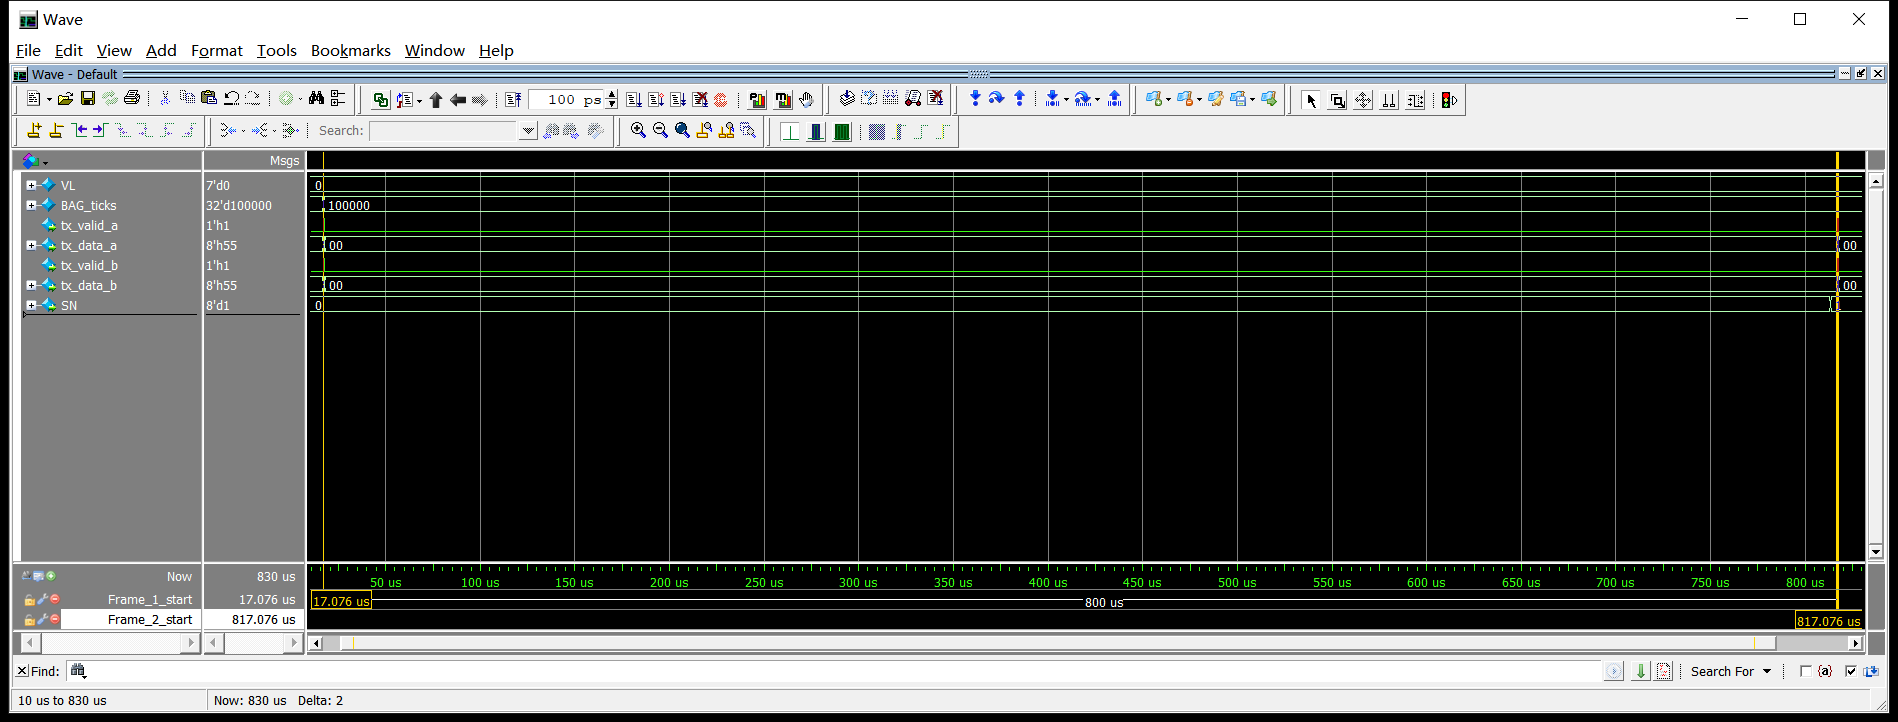
\includegraphics[width=\linewidth]{../../sim/wave/png/tx_bag.png}
\caption[同一 VL 发送间隔的原始波形]{同一 VL 发送间隔的 ModelSim 原始波形：光标 \code{Frame_1_start = 17.132}~µs 与 \code{Frame_2_start = 817.132}~µs 严格相隔 800.000~µs（100,000 拍）。}
\label{fig:capture-bag}
\end{figure}

\clearpage

\section{应用消息与双网发送}

图~\ref{fig:capture-tx} 展示应用口写入与 A、B 两网发送的时序，以及发送起点附近的字节变化。在图~\ref{fig:capture-tx}(a) 中，时间窗口为 686.272--689.372~µs，光标 \code{GMII_start = 688.572}~µs 处 A、B 两网同拍起发前导码 \code{55}；在图~\ref{fig:capture-tx}(b) 放大窗口（688.564--688.892~µs）中，两网帧头仅源 MAC 地址中的网络号不同（A 网为 \code{20}、B 网为 \code{40}）。

\begin{figure}[H]\centering
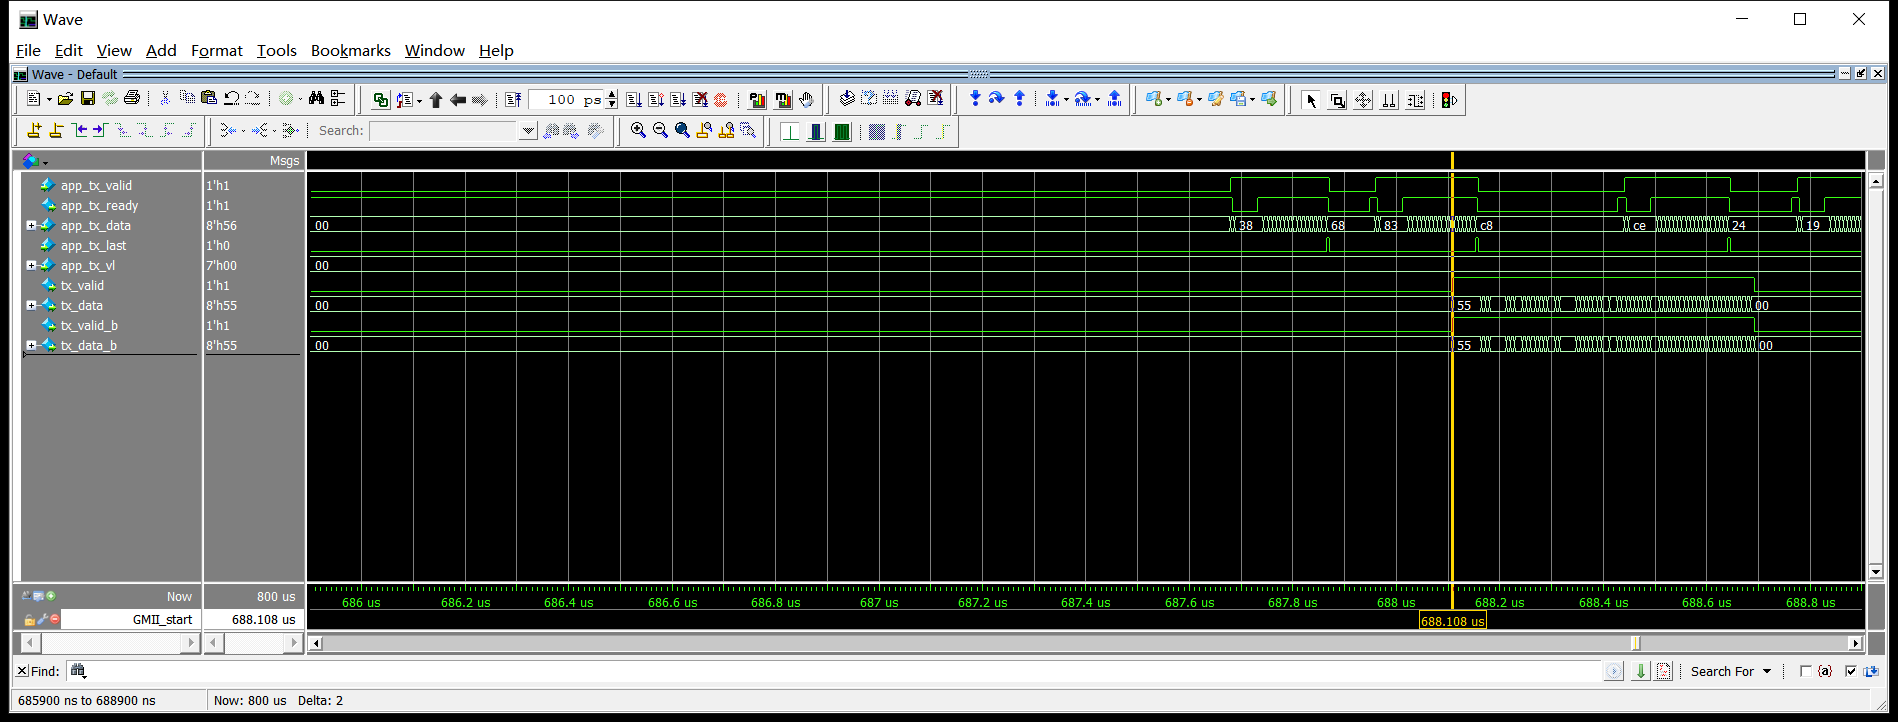
\includegraphics[width=\linewidth]{../../sim/wave/png/tx_dual_1.png}
\par\smallskip
{\small (a) 应用口写入与双网发送整体时序（窗口 686.272--689.372~µs，光标 \code{GMII_start = 688.572}~µs 两网同拍起发）\par}
\medskip
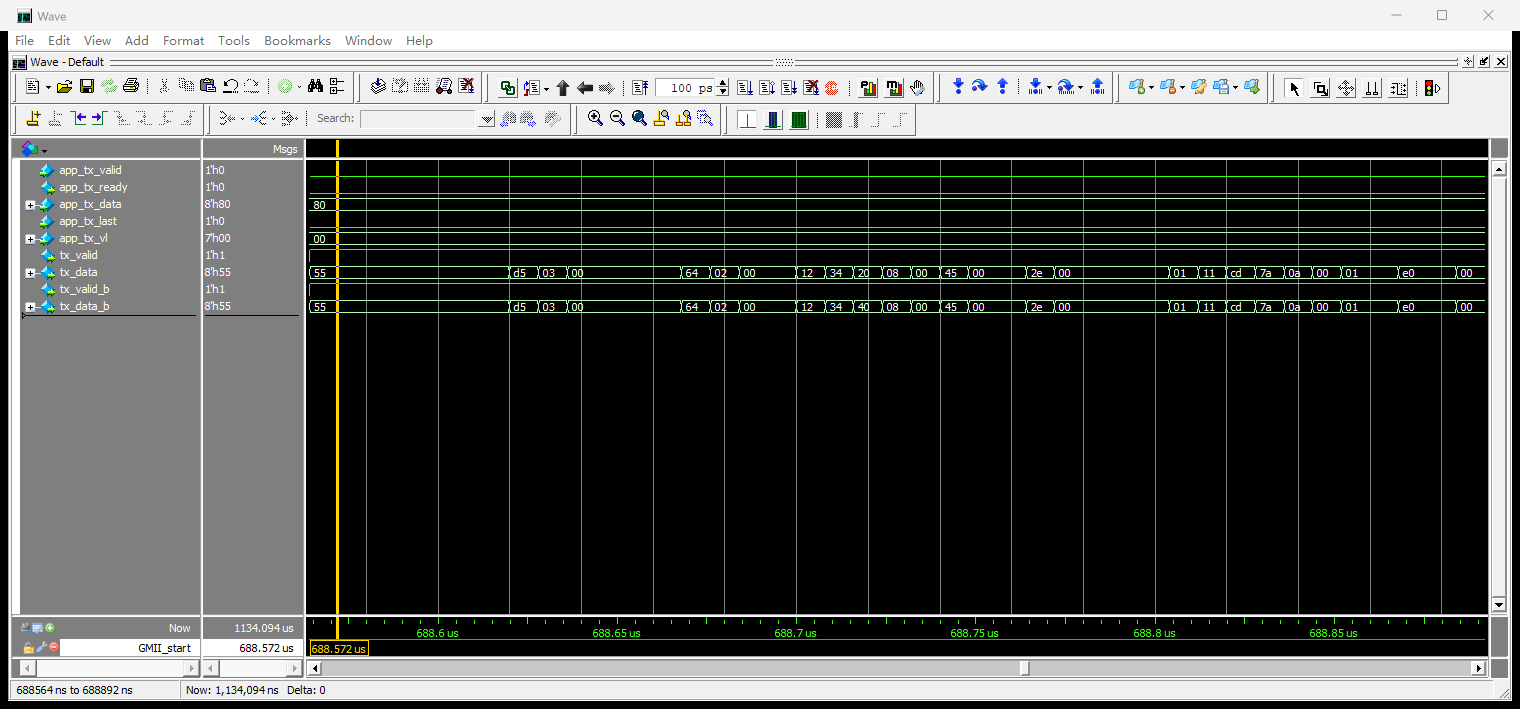
\includegraphics[width=\linewidth]{../../sim/wave/png/tx_dual_2.png}
\par\smallskip
{\small (b) A、B 两网发送起点与帧头字节放大（窗口 688.564--688.892~µs，源 MAC 分别为 \code{20} 与 \code{40}）\par}
\caption[应用消息与双网发送的原始波形]{应用消息与双网发送的 ModelSim 原始波形：光标 \code{GMII_start = 688.572}~µs 处两网同拍开始发送前导码 \code{55}。}
\label{fig:capture-tx}
\end{figure}

\clearpage
\section{双网副本接收与去重}

图~\ref{fig:capture-rm} 展示先到副本的应用交付，以及晚到副本触发的冗余丢弃事件。在图~\ref{fig:capture-rm}(a) 中，时间窗口为 3016.794--3017.104~µs，光标 \code{A_delivered = 3016.844}~µs 处先到的 A 网副本交付应用（\code{app_rx_net = 0}）；在图~\ref{fig:capture-rm}(b) 中，时间窗口为 3032.408--3032.668~µs，光标 \code{B_duplicate = 3032.628}~µs 处晚到 15.784~µs 的 B 网副本触发 \code{ev_rm_drop} 脉冲并被丢弃。

\begin{figure}[H]\centering
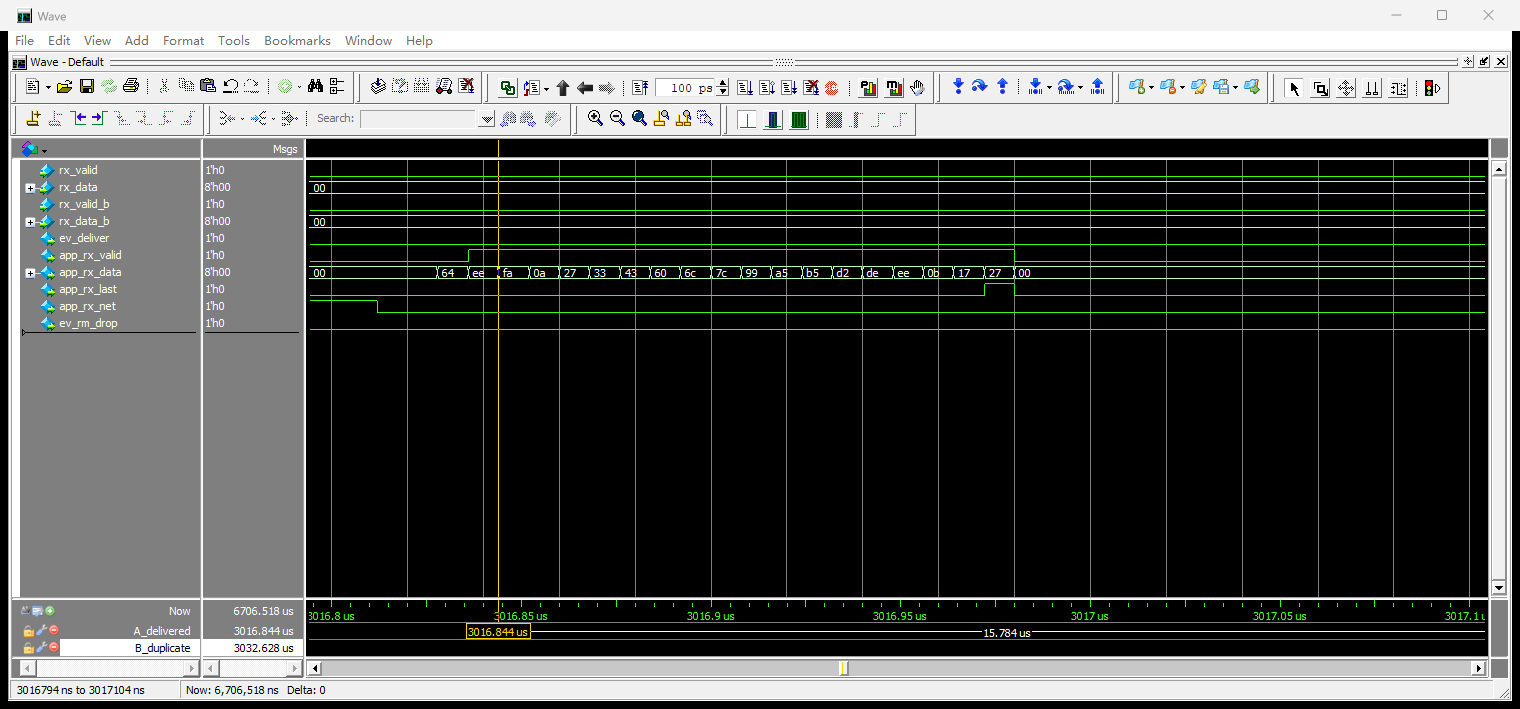
\includegraphics[width=\linewidth]{../../sim/wave/png/rx_redundancy_1.png}
\par\smallskip
{\small (a) A 网副本触发交付事件并向应用口输出消息（光标 \code{A_delivered = 3016.844}~µs）\par}
\medskip
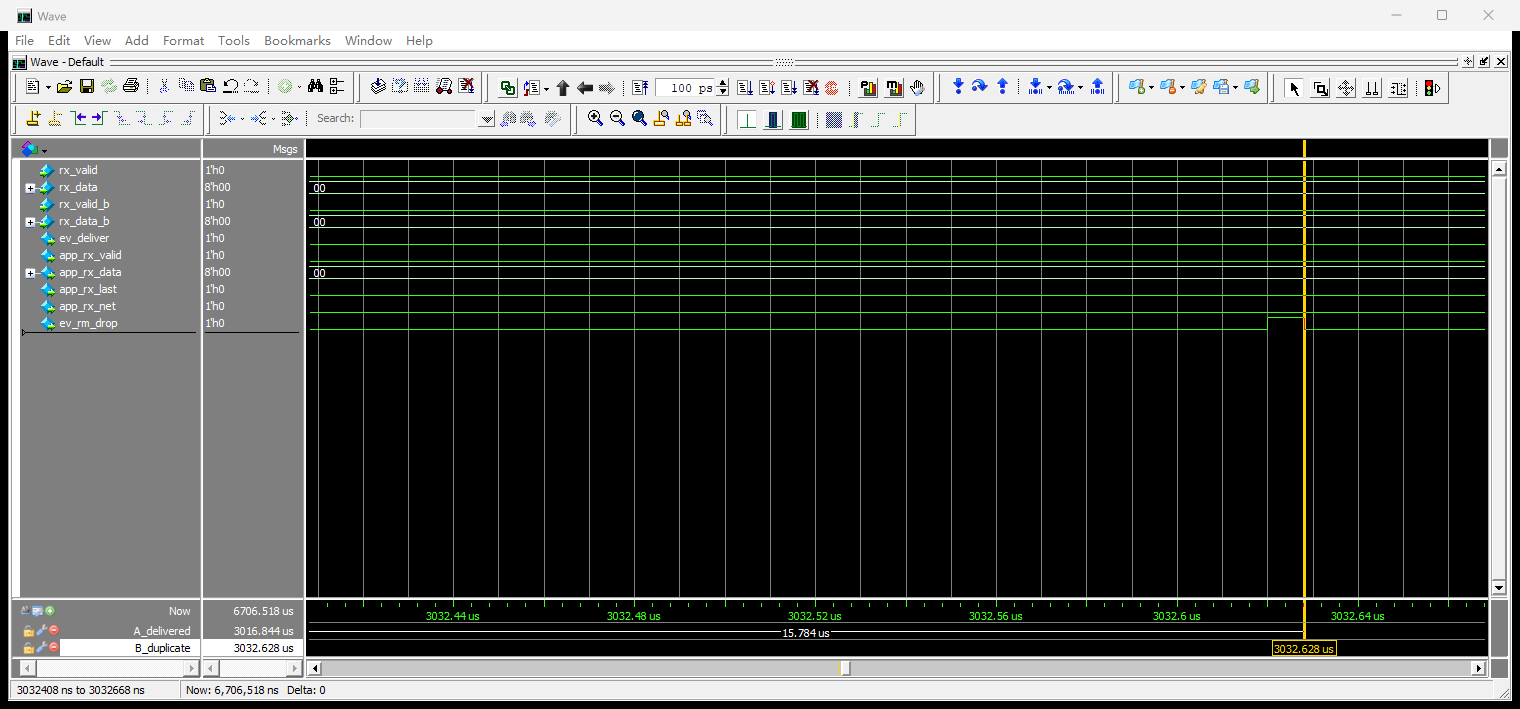
\includegraphics[width=\linewidth]{../../sim/wave/png/rx_redundancy_2.png}
\par\smallskip
{\small (b) 晚到 15.784~µs 的 B 网副本触发 \code{ev_rm_drop} 丢弃（光标 \code{B_duplicate = 3032.628}~µs）\par}
\caption[双网副本接收与去重的原始波形]{双网副本接收与去重的 ModelSim 原始波形：A 网副本先到交付，晚到 15.784~µs 的 B 网副本被冗余管理丢弃。}
\label{fig:capture-rm}
\end{figure}

\clearpage
\section{FCS 错误检测与计数读回}

图~\ref{fig:capture-fcs} 展示 FCS 错误事件、计数变化和配置口的独立读请求。在图~\ref{fig:capture-fcs}(a)（时间窗口 798.620--799.920~µs）中，光标 \code{FCS_error = 799.620}~µs 处 A 网坏帧拒收，\code{count_a_fcs} 由 0 增至 1；在图~\ref{fig:capture-fcs}(b)（时间窗口 973.396--973.436~µs）中，测试平台于 973.404~µs 发起对地址 \code{0x49} 的真实读请求，两拍后 973.420~µs 返回计数 1（\code{cfg_rvalid = 1}、\code{cfg_rdata = 1}）。

\begin{figure}[H]\centering
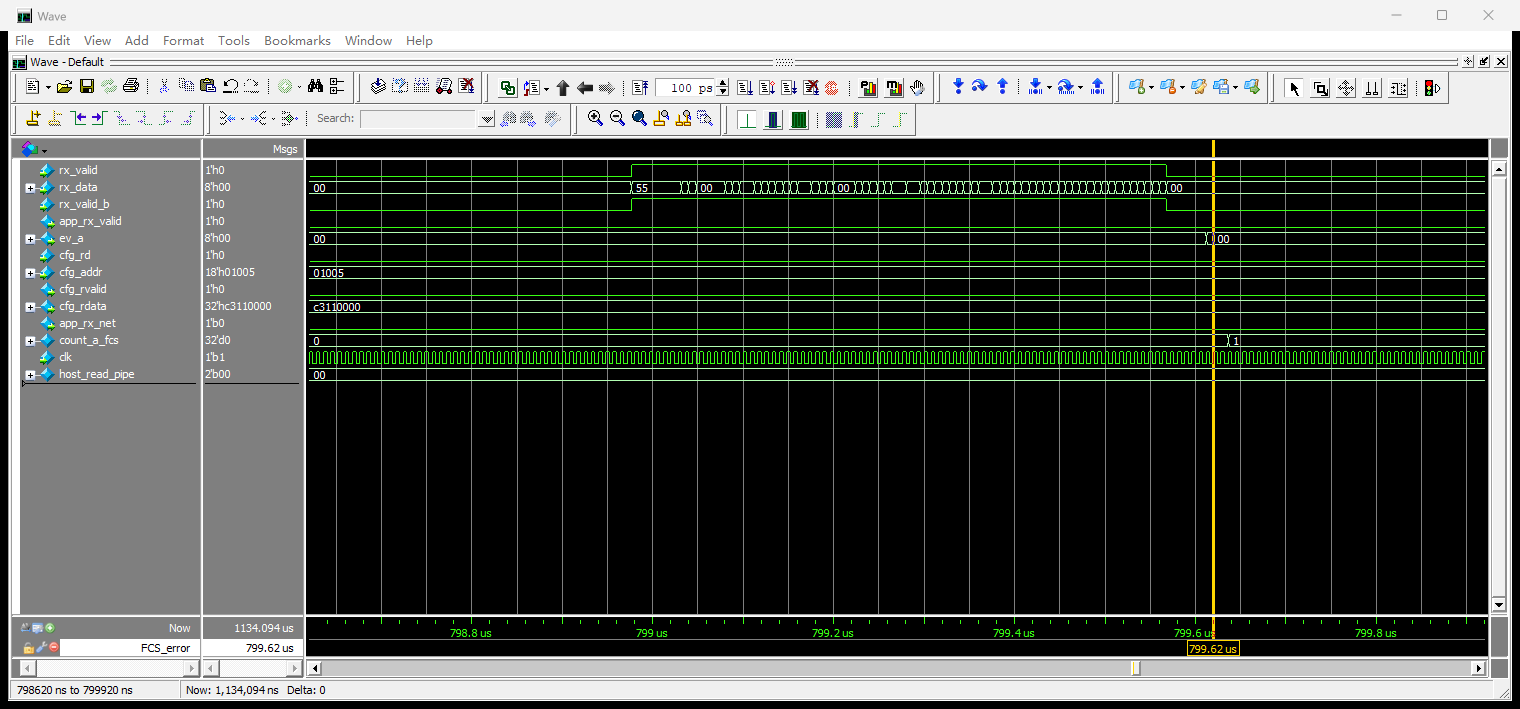
\includegraphics[width=\linewidth]{../../sim/wave/png/rx_fcs_error_1.png}
\par\smallskip
{\small (a) \code{ev_a_fcs_error} 脉冲与 \code{count_a_fcs} 从 0 增至 1（光标 \code{FCS_error = 799.620}~µs）\par}
\medskip
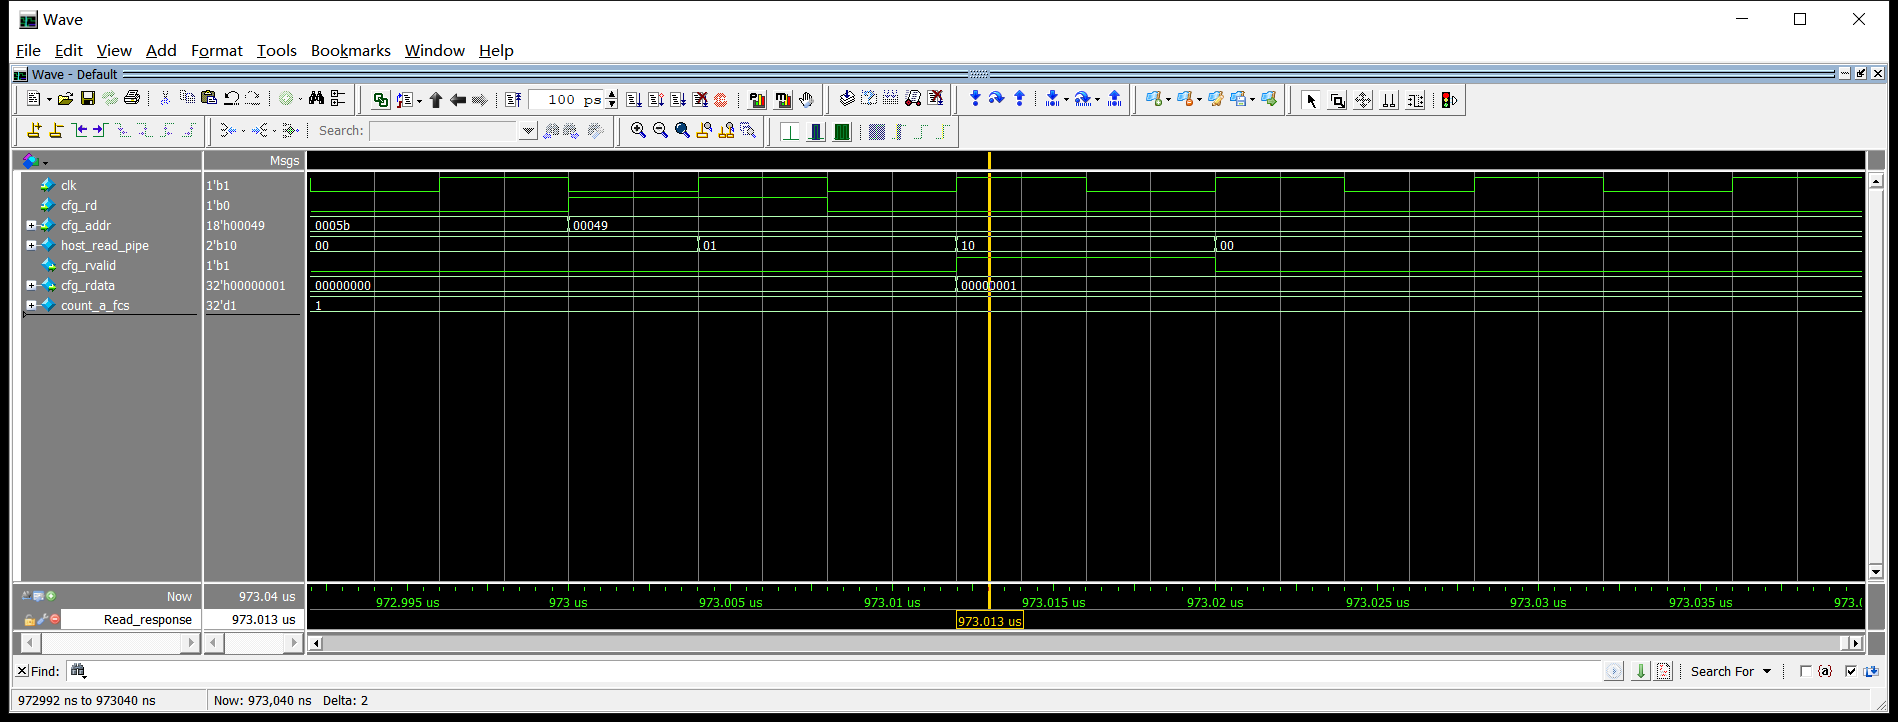
\includegraphics[width=\linewidth]{../../sim/wave/png/rx_fcs_error_3.png}
\par\smallskip
{\small (b) 配置口读取地址 \code{0x49}（973.404~µs 发起请求，两拍后 973.420~µs 返回计数 1）\par}
\caption[FCS 错误检测与计数读回的原始波形]{FCS 错误检测与计数读回的 ModelSim 原始波形：799.620~µs 检测到 A 网 FCS 错误并使计数加 1，配置口读请求经两拍精确返回该值。}
\label{fig:capture-fcs}
\end{figure}

\clearpage
\section{SNMP Get 请求与响应}

图~\ref{fig:capture-snmp} 展示管理请求到达代理以及代理从 A、B 两网回送响应的时序。在图~\ref{fig:capture-snmp}(a)（窗口 525.944--526.284~µs）中，光标 \code{Get_request = 525.964}~µs 请求到达；在图~\ref{fig:capture-snmp}(b)（窗口 538.604--538.948~µs）中，光标 \code{Get_response = 538.628}~µs 代理从 A、B 两网同拍回送响应，距请求到达严格相隔 12.664~µs。

\begin{figure}[H]\centering
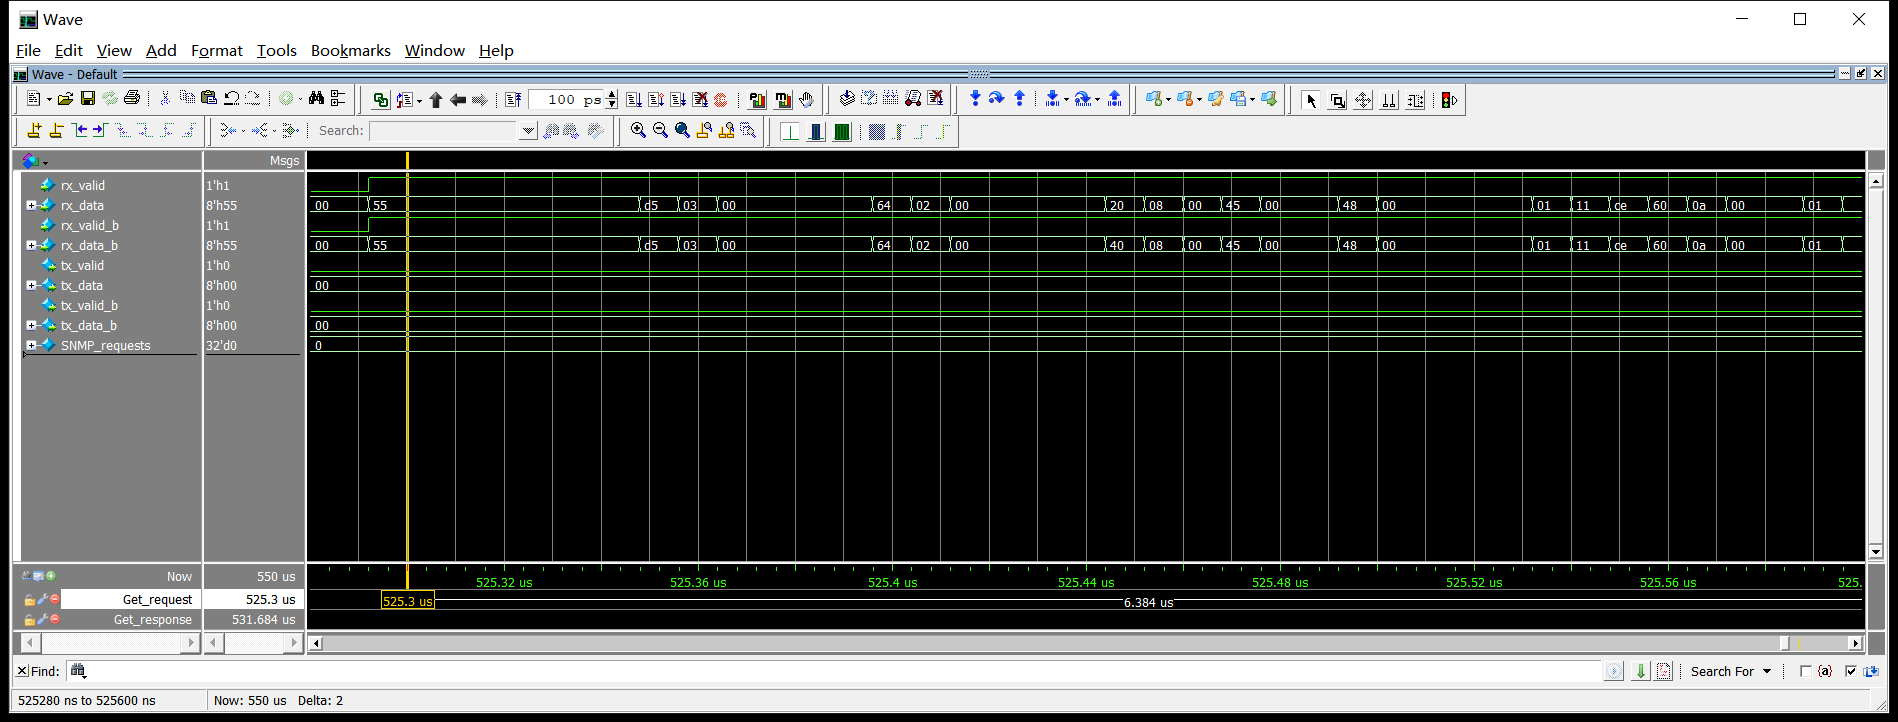
\includegraphics[width=\linewidth]{../../sim/wave/png/snmp_get_1.png}
\par\smallskip
{\small (a) Get 请求经 A、B 两网到达代理（光标 \code{Get_request = 525.964}~µs）\par}
\medskip
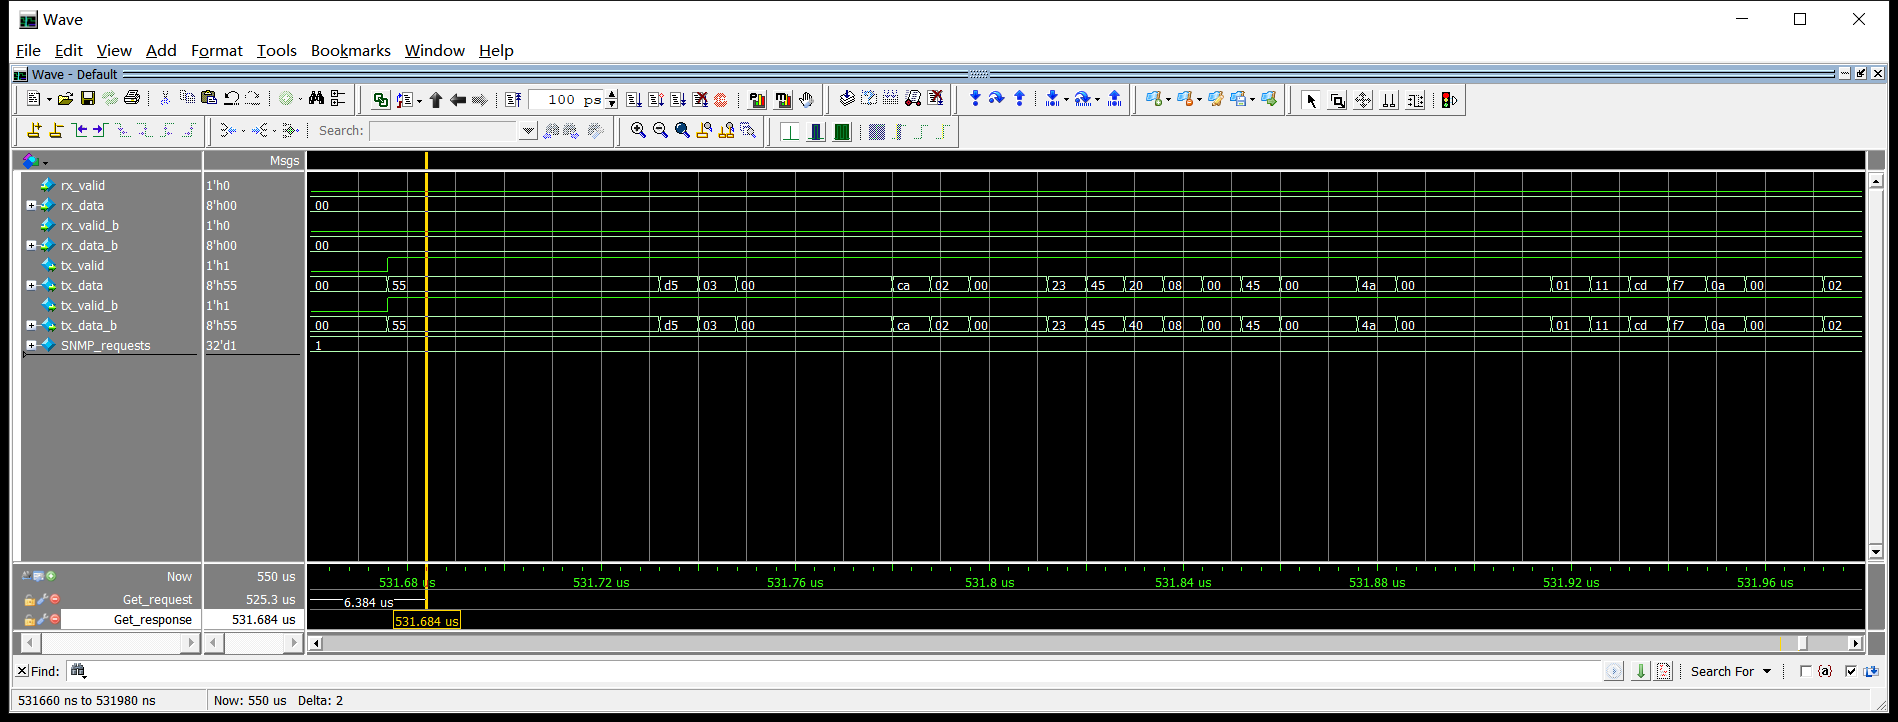
\includegraphics[width=\linewidth]{../../sim/wave/png/snmp_get_2.png}
\par\smallskip
{\small (b) 代理从 A、B 两网同拍发送响应（光标 \code{Get_response = 538.628}~µs，距请求相隔 12.664~µs）\par}
\caption[SNMP Get 请求与响应的原始波形]{SNMP Get 请求与响应的 ModelSim 原始波形：请求经双网到达代理，处理后经双网同拍发出响应，间隔 12.664~µs。}
\label{fig:capture-snmp}
\end{figure}

\clearpage
\section{超长消息 IPv4 分片发送与按序重组}\label{sec:cap-frag}

在 ModelSim 中执行 \code{do sim/wave/frag.do}（或 \code{python sim/wave/export.py --scene frag}），对 \code{VL 0x0103} 单条 8192~B 消息拆分为 6 个 IPv4 分片（片偏移依次为 0、1472、2944、4416、5888、7360~B，前 5 片 \code{MF=1}、末片 \code{MF=0}，相邻分片间隔 1~ms BAG）经 A、B 两网同拍发送并一次完整重组交付 8194~B（2~B VLID + 8192~B 载荷）的波形进行全景与细节观测。

图~\ref{fig:capture-frag} 汇集了该场景的 ModelSim 原始波形截图：

\begin{figure}[H]\centering
  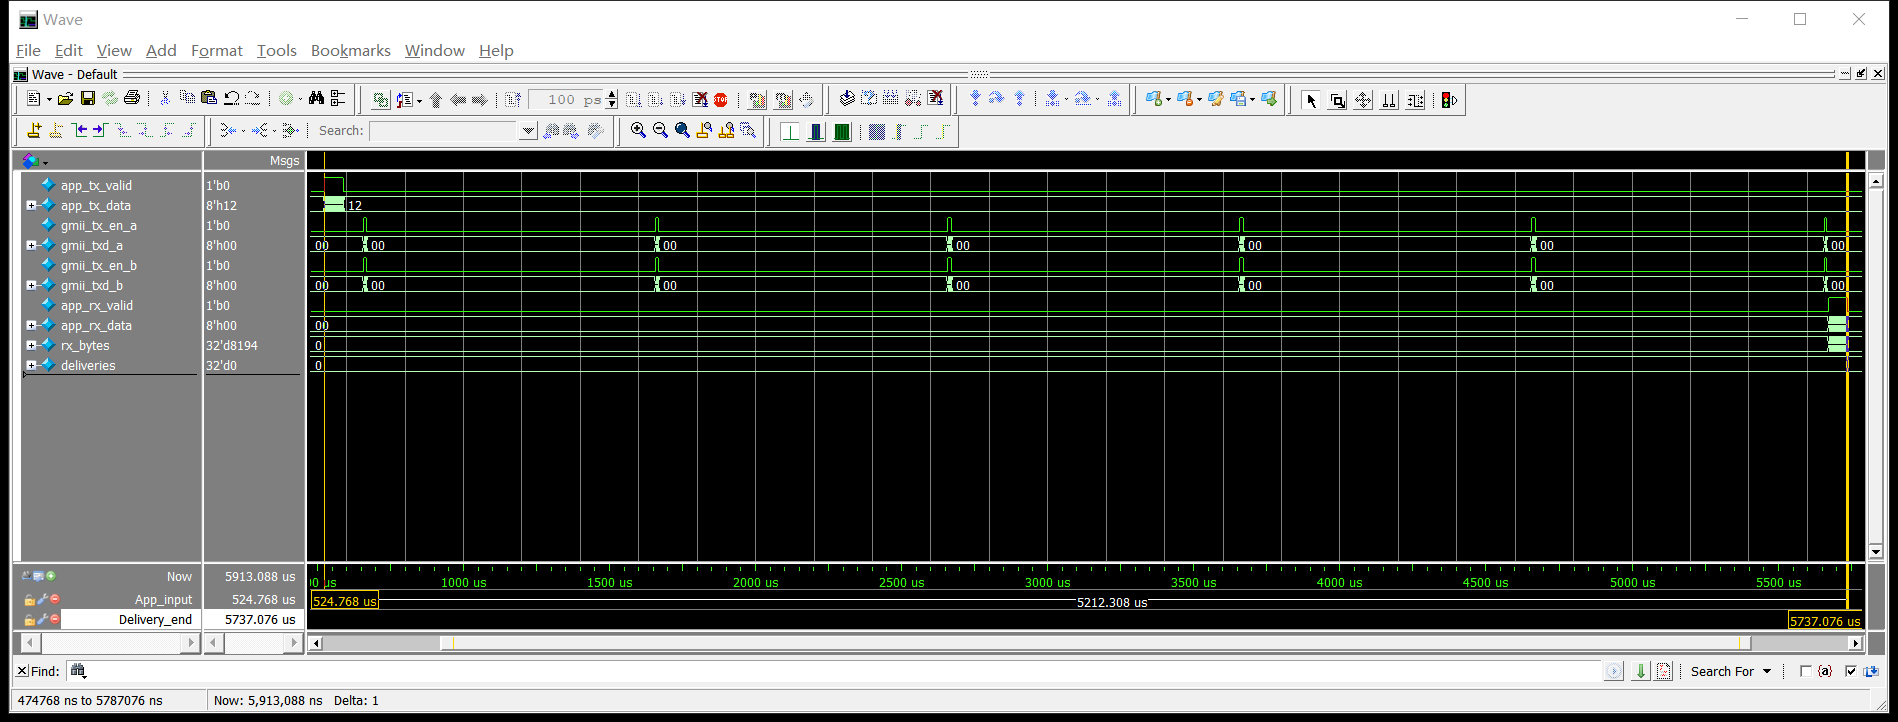
\includegraphics[width=\linewidth,height=0.20\textheight,keepaspectratio]{../../sim/wave/png/frag_1.png}
  \par\smallskip
  {\small (a) 8192~B 消息 6 分片发送与重组交付全程总览（窗口 474.768--5787.076~µs，跨度 5212.308~µs）\par}
  \medskip
  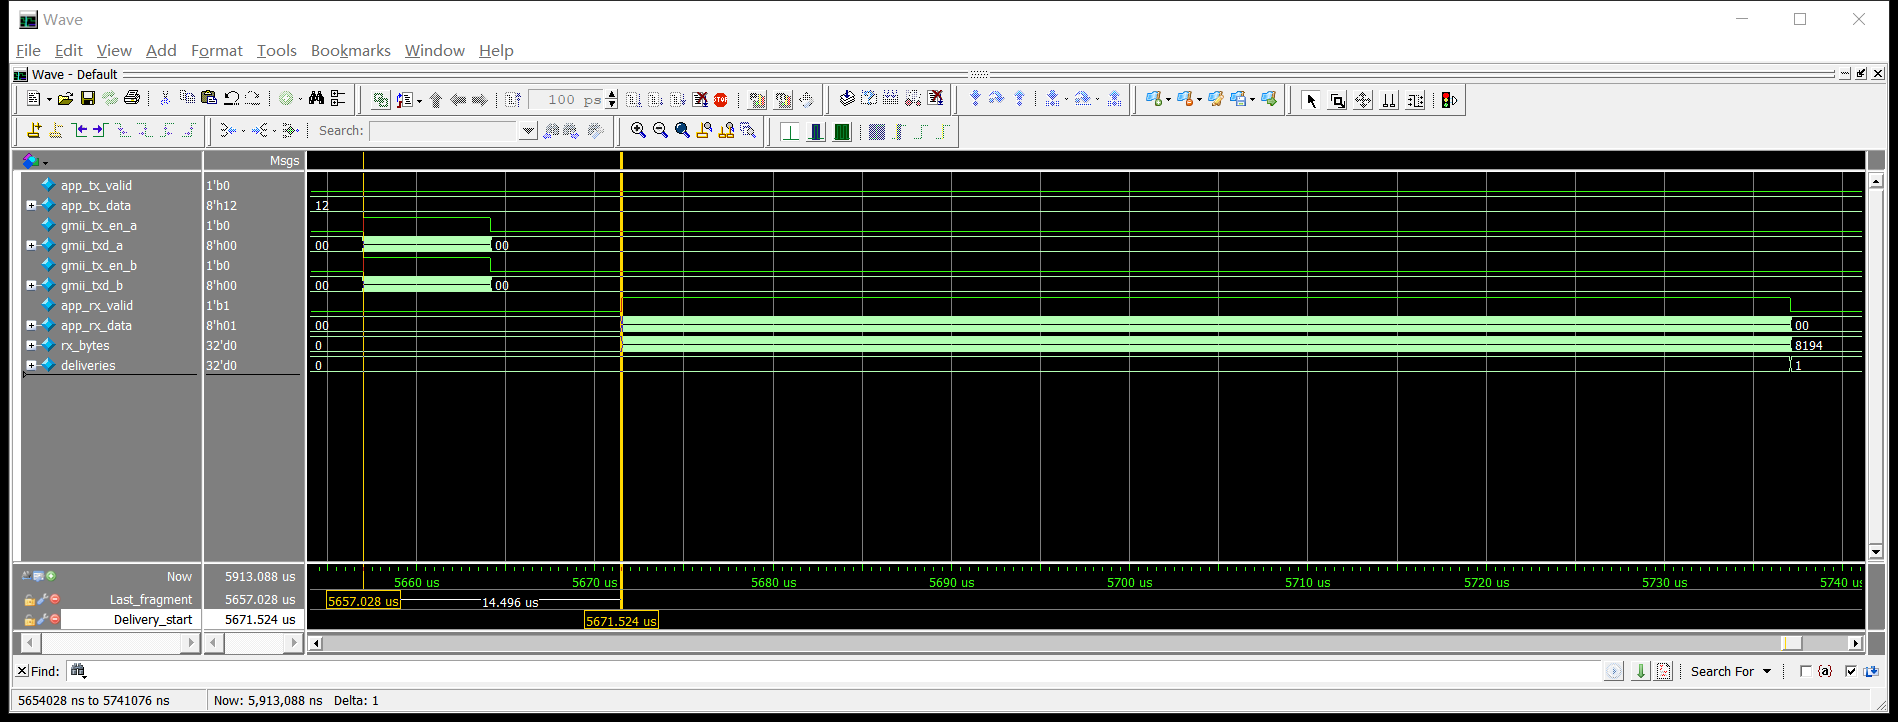
\includegraphics[width=\linewidth,height=0.20\textheight,keepaspectratio]{../../sim/wave/png/frag_2.png}
  \par\smallskip
  {\small (b) 末片 5657.028~µs 到达后 5671.524~µs 启动连续交付，\code{rx_bytes} 精确计至 8194\par}
  \medskip
  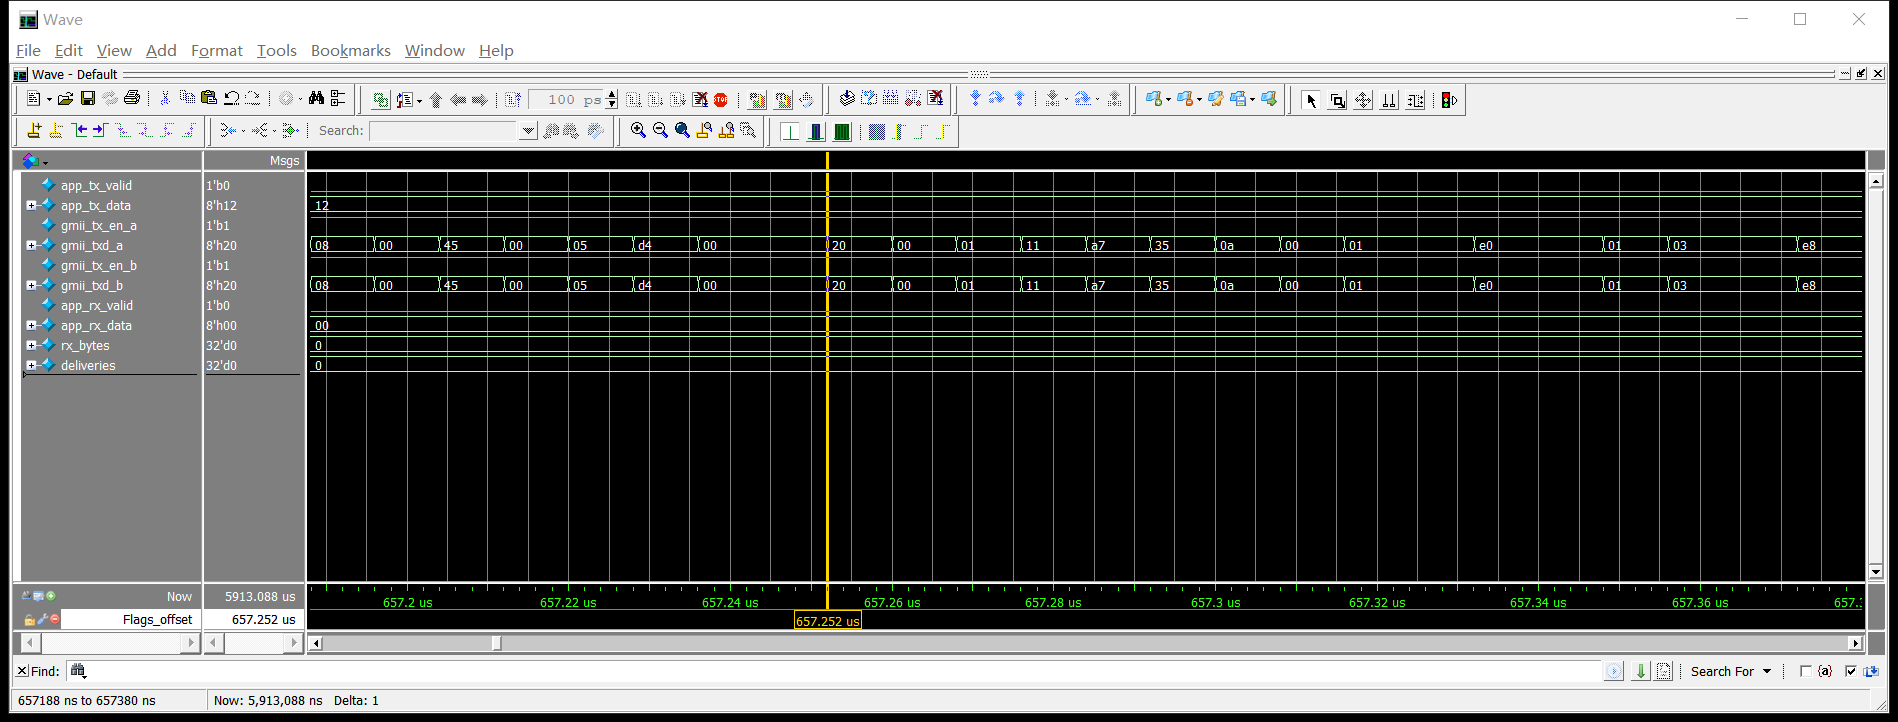
\includegraphics[width=\linewidth,height=0.18\textheight,keepaspectratio]{../../sim/wave/png/frag_3.png}
  \par\smallskip
  {\small (c) 首片 IPv4 报头字节放大，光标 657.252~µs 处标志与片偏移字段为 \code{20 00}（\code{MF=1}，偏移 0）\par}
  \caption[超长消息 IPv4 分片发送与按序重组原始波形]{超长消息 IPv4 分片发送与按序重组 ModelSim 原始波形：(a) 激励起点 524.768~µs 至交付结束 5737.076~µs 的 6 分片全流程；(b) 末片到达后一次完整交付 8194 字节；(c) 首片 IP 头 \code{MF=1} 与偏移 0。}\label{fig:capture-frag}
\end{figure}
